\documentclass{standalone}
\usepackage{tikz}
\usetikzlibrary{arrows,shapes,positioning,shadows,trees}

\begin{document}
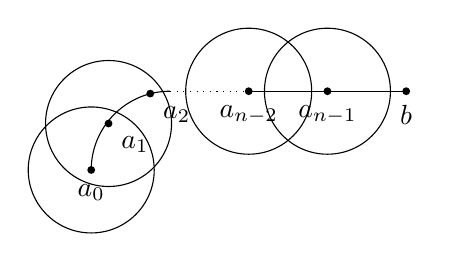
\begin{tikzpicture}
    \draw (-1,0) arc (180:90:1);
    \draw[dotted] (0,1) -- (1,1);
    \draw (1,1) -- (3,1);
    \node[fill,circle,inner sep=1pt,label=below:$a_0$] at (-1,0) {};
    \node[fill,circle,inner sep=1pt,label=below right:$a_1$] at (-0.78,0.59) {};
    \node[fill,circle,inner sep=1pt,label=below right:$a_2$] at (-0.25,0.97) {};
    \node[fill,circle,inner sep=1pt,label=below:$a_{n-2}$] at (1,1) {};
    \node[fill,circle,inner sep=1pt,label=below:$a_{n-1}$] at (2,1) {};
    \node[fill,circle,inner sep=1pt,label=below:$b$] at (3,1) {};
    \draw (-1, 0) circle (0.8);
    \draw (-0.78, 0.59) circle (0.8);
    \draw (1, 1) circle (0.8);
    \draw (2, 1) circle (0.8);
\end{tikzpicture}
\end{document}